%LET'S GO TEAM!!! ONE LESS SECTION
%We are unstoppppable --> DAB DAB DAB
The design of the constellation depends mainly on the coverage that a single satellite can provide. The parameters that define this coverage need to be deeply studied since their influence in the final constellation design is very significant. They can be listed below:

\paragraph{Satellite - Ground Visibility main parameters}
\begin{itemize}
\item \textbf{Footprint:} Defined as the region of Earth where a single satellite can
be seen. Details on its computation found in [{REF TO ANNEX I. Section 2.1}]. 
\item \textbf{Elevation Angle:} The angle between the Ground Station beam pointing to the satellite and the horizontal local plane. Usually described as the minimum elevation angle necessary to avoid atmospheric absortion of the signal. A deep analysis on this influence and the implications of the constellation design can be found in [{REF TO ANNEX I. Section 2.2}]. The geometry of the setup can be seen in figure \ref{fig:AngleSSatFoot}
\item \textbf{Minimum Plane Inclination: } If the goal is to provide global coverage, then there is a minimum latitude in which the satellites can orbit. This minimum inclination is assessed in [{REF TO ANNEX I. Section 2.3}].
\end{itemize}

\paragraph{Satellite to Satellite Visibility\\}
In this case, the conditions are set by direct linear communication between the two satellites. The details on the determination of this limitation is found in [{REF TO ANNEX I. Section 2.4}].

\begin{figure}[H] %[b] % h / H / b / t
	\centering
	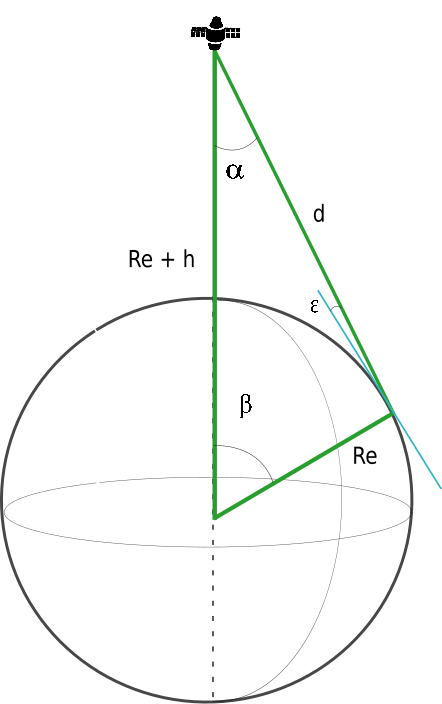
\includegraphics[width=.3\textwidth]{./fig-Ch2-OrbitalCoverage/AngleSSatFoot.png}
	\caption{Single satellite coverage geometry}
	\label{fig:AngleSSatFoot}
	
\end{figure}